\chapter{Inter-Island Trade Organisation (IITO)}

\section{Design}
\label{sec:IITO:Design}

The role of IITO is to facilitate inter-island communication and to enable the acts of giving and receiving gifts. In a more complete and realistic multi-agent simulation, unrestricted communication between the islands could have been considered, where islands could communicate with one another in an unconstrained manner. However, such a communication style would also assume the fact that the islands are rather complex agents which are able to undertake considerably sophisticated actions. Therefore, for the coursework, specific forms of communication were chosen to sensibly restrict the island complexity while still allowing for interesting interactions between the islands to take place.

\subsection{Inter-Island Communication}  
\label{subsec:IITO:inter_island_communication}

Islands which can communicate separately from the main governing body level of interactions (i.e. IIGO) makes more complex island behaviour possible. With the implemented systems, islands can:

\begin{itemize}
    \item Form a group with other islands for collective foraging.
    \item Decide where their foraging group will forage.
    \item Inform other islands of the amount they intend to to donate to the common pool.
    \item Share voting history with other islands.
    \item Share tax amount history with other islands.
    \item Inform other islands of the amount of resources they currently have in their private pool.
\end{itemize}

\textbf{Team Foraging}: Allows islands to decide between each other whether they will forage together and where they will forage. In this way, islands can cooperate with the others that they trust while avoiding other islands that they deem to have misbehaved or broken rules in the past. If islands suspect that some specific islands have deliberately freeloaded in the previous forages, they may also want to avoid foraging with such islands that have contributed less than what they were supposed to.

\textbf{Common Pool Donations}: Allows islands to broadcast how much they plan to donate to the common pool and let them declare to the other islands if they plan to donate more than the specified tax amount put forward by the President as a form of virtue signalling. This may help an island redeem itself if it had previously lost trust. Note that an island can lie about the amount it will donate to the common pool if it is trying to maliciously gain favour.

\textbf{Voting History}: Islands can request voting history from other islands or provide their own one unprompted. This interaction enables islands to verify whether the Speaker has been honest when counting the votes for a previously held election. Note that the islands can lie in the voting history that they provide, meaning that the islands may want to only take heed of information from those islands that they already trust.

\textbf{Tax History}: Similarly to providing and requesting voting history, islands can request taxation history (i.e. how much the islands were told to contribute in the form of tax by the President) from other islands. Note that an island may choose not to provide this tax history or it can be dishonest about it. If the islands report the true level of taxation, this interaction allows islands to form an opinion about whether the President has decided on a fair\footnote{Note that this fairness metric will be unique to each island, meaning that it is subjective.} amount of taxation.

\textbf{Current Resources}: Islands are also able to share the value of the resources that they currently have in their private pool. This information may guide islands when making decisions regarding gifts (Section~\ref{subsec:IITO:gifting}). For example, if an island requests a gift because they are low on resources, the island receiving the request may want to ask how many resources the requesting island has. This can also give an island an indication of the overall level of richness in the archipelago. Similarly to sharing the intended common pool donations along with voting and tax history, the islands can decide not to report or lie about their current amount of resources.

\subsection{Gifting}  
\label{subsec:IITO:gifting}  

If an island is struggling and requires some additional amount of resources to survive, it may ask the President for an allocation from the common pool but the President may reject this request. The struggling island would still be able to take resources from the common pool if rejected, but law-abiding islands would probably want to avoid such disobedience. To allow islands to still request an additional amount of resources from the other islands, the \textbf{gifting} action is an option. Islands may accept the gift requests if they wish to improve their standing with the requesting islands. They can also accept the gift requests of those whose survival is deemed to be essential for the future of the archipelago. When requesting, giving or receiving a gift, the island can specify a reason for this action, which gives islands more information about the gifting transaction. For example, a requesting island may want to specify that they will move to a critical state in the next round if they do not receive the gift, or an offering island may want to specify that the gift is meant as a reward for successful disaster forecasting.

Islands are also able to offer gifts without a request being made, meaning they can reach out to other islands if they want to boost their popularity.

\section{Implementation}
\label{sec:IITO:Implementation}

\subsection{Server Client Infrastructure}
\label{subsec:IITO:server_client_infrastructure}  

During a turn, once IITO has started, a series of sessions are run, and the conclusion of all these sessions indicates that the IITO is also complete. In the current implementation, these sessions include gift giving and common pool donations, and they all follow the same client-server interaction format\footnote{Server and Client are defined in Definition~\ref{def:server} and Definition~\ref{def:client} respectively}. The server acts an intermediary for all client to client communication, and prompts clients to make decisions or formulate messages during the session. At each stage in a session the server compiles a list of messages from the clients, following that sessions' protocols, and then uses that list as input for the next stage. While a bit abstract this is better explained through an example.

\subsection{Gifting Session}
\label{subsec:IITO:gifting_session} 

There are four phases to the gifting sessions: Gift requests, gift offers, gift responses and updating gift history. Each part is further explained below and Figure~\ref{fig:IITO:gifting_session_diagram} shows the interactions a single client will have with the server over the session.
\begin{itemize}
    \item \textbf{Gift Requests}: This part collects the gift requests of all clients. These requests include an amount the client wants and who they wish to request from.
    \item \textbf{Gift Offers}: Here we give the clients any requests that are directed to them and then collects the gift offers from each client. These offers include an amount the client wished to gift and to whom the gift is being offered.
    \item \textbf{Gift Responses}: Here we provide the client with all the offers directed towards them and prompts them to respond to each of these offers. These responses contain the amount the client wishes to accept and a reason for their decision.
    \item \textbf{Updating Gift History}: In this stage client's are told of the outcome of any offers they gave out. A client is told whether or not an offer has been accepted, the reason for the rejection or acceptance and also the amount the receiver wishes take. For example Team 1 may offer $100$ resources to Team 2, but Team 2 may only want take $50$. The implemented system allows for such behaviour.
\end{itemize}

\begin{figure}[!htb]
    \centering
    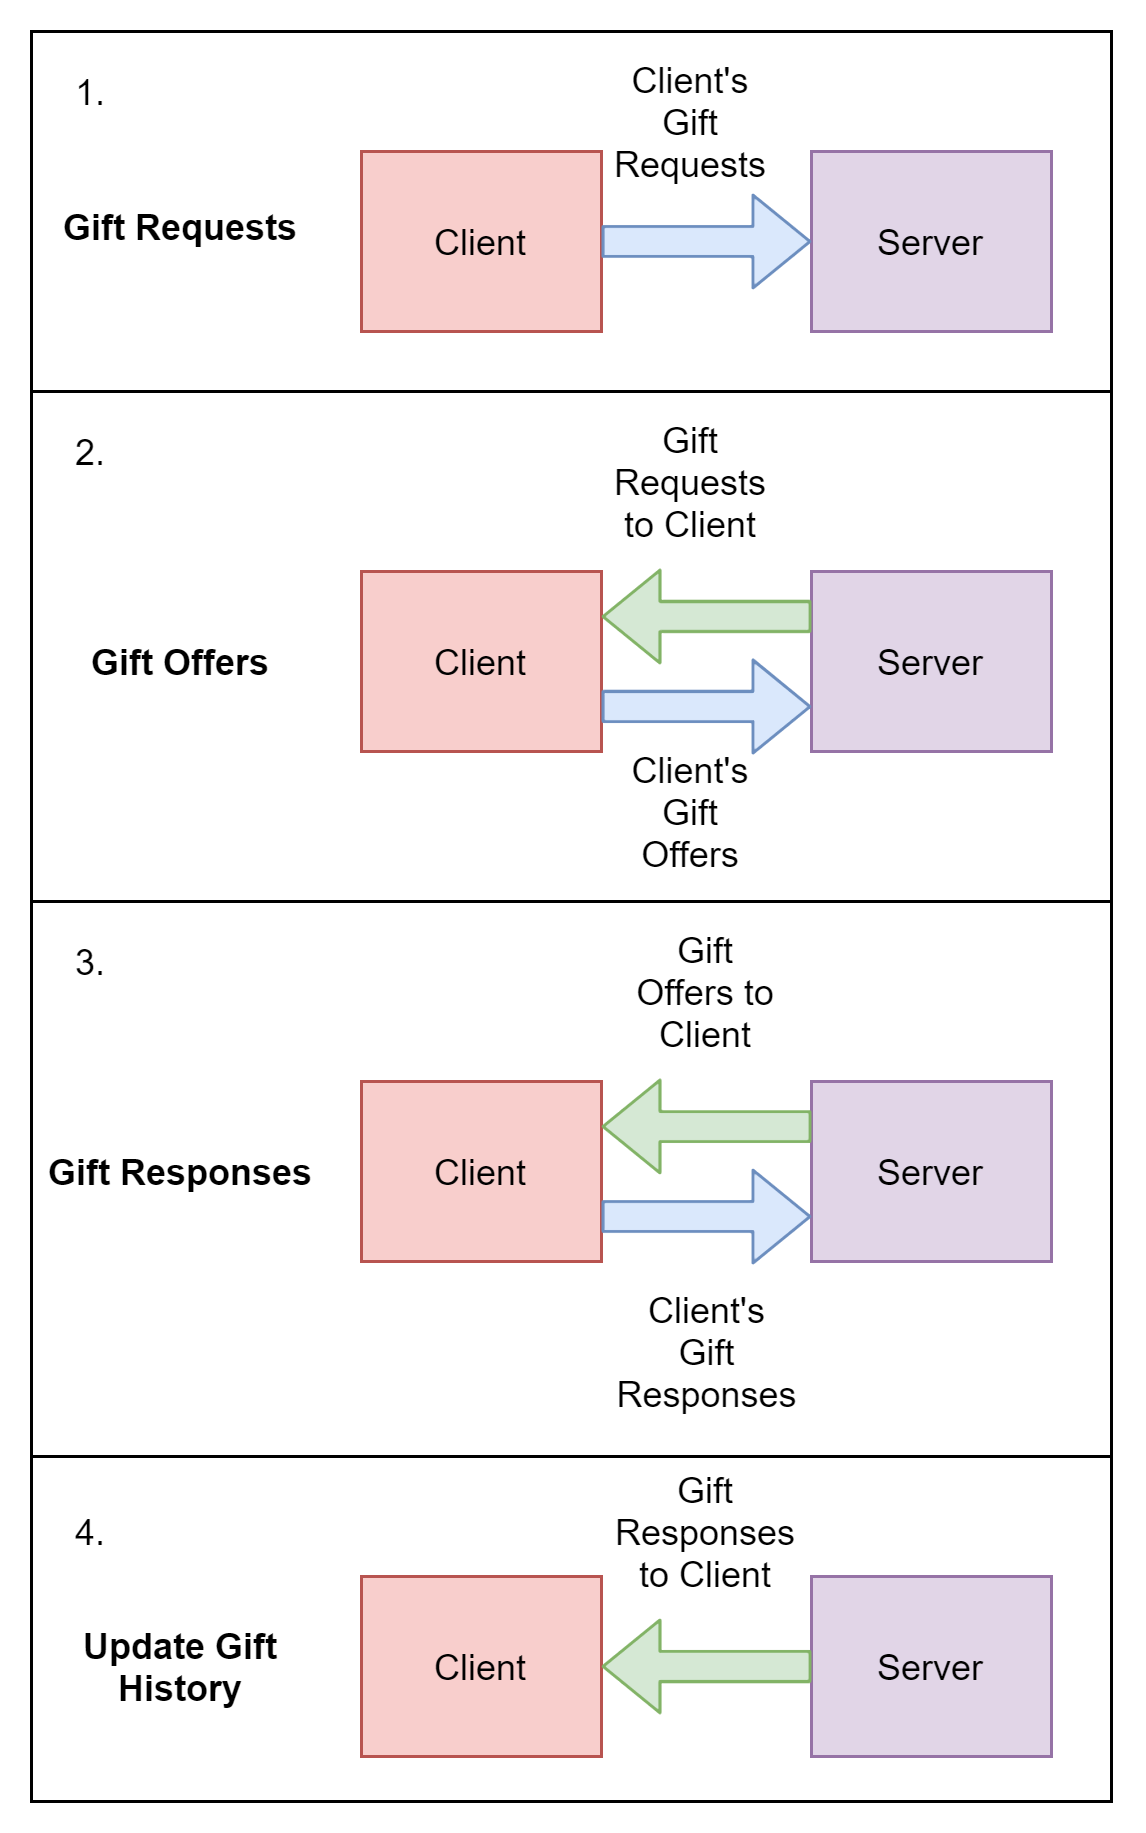
\includegraphics[width=0.6\textwidth]{06_iito/images/gifting_diagram.png}
    \caption{Overview of client-server interactions in gifting session.}
    \label{fig:IITO:gifting_session_diagram}
\end{figure}

